\begin{pastexam}[label={px:ntu-109-esoe-ds-06}]{臺大工科海洋所 109 學年度 第 6 題}
（作圖、追蹤）

\textbf{(15 \%)} Weighted graph.
\begin{enumerate}[label=(\alph*)]
\item (8 \%) Draw a simple, connected, undirected, weighted graph with 8 vertices and 16 edges,
each with unique edge weights.
\item (7 \%) Find the minimum spanning tree of the graph.
\end{enumerate}
\end{pastexam}

\begin{pastsoln}
\textbf{(a)} 圖由自己設計，只要符合四個條件：簡單（沒有自環、沒有重邊）、連通、無向、$8$ 個頂點
$16$ 條邊而且權重兩兩不同。 $8$ 個頂點的簡單圖最多 $\binom{8}{2} = 28$ 條邊，$16$ 條做得到；連通
至少要 $7$ 條，也沒問題。 下面用內外兩個正方形：外圈 $a, b, c, d$、內圈 $e, f, g, h$，外圈 $4$ 條、
內圈 $4$ 條、內外對應的 $4$ 條，再加上每個梯形的一條對角線 $4$ 條，共 $16$ 條，權重用
$1$ 到 $16$ 各一次。 這樣畫沒有邊交叉，權重容易看清楚。

\begin{center}
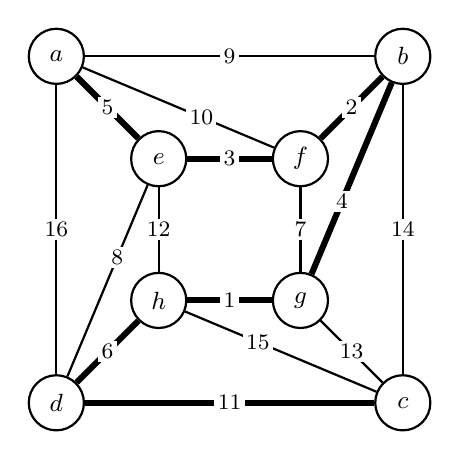
\begin{tikzpicture}[
    v/.style={circle, draw, thick, minimum size=7mm, inner sep=0pt, font=\small},
    w/.style={fill=white, inner sep=1.2pt, font=\footnotesize},
    e/.style={thick}, t/.style={line width=2.2pt}]
\node[v] (a) at (0,4.4) {$a$};
\node[v] (b) at (4.4,4.4) {$b$};
\node[v] (c) at (4.4,0) {$c$};
\node[v] (d) at (0,0) {$d$};
\node[v] (e) at (1.3,3.1) {$e$};
\node[v] (f) at (3.1,3.1) {$f$};
\node[v] (g) at (3.1,1.3) {$g$};
\node[v] (h) at (1.3,1.3) {$h$};
\draw[e] (a) -- node[w] {9} (b);
\draw[e] (b) -- node[w] {14} (c);
\draw[t] (c) -- node[w] {11} (d);
\draw[e] (d) -- node[w] {16} (a);
\draw[t] (e) -- node[w] {3} (f);
\draw[e] (f) -- node[w] {7} (g);
\draw[t] (g) -- node[w] {1} (h);
\draw[e] (h) -- node[w] {12} (e);
\draw[t] (a) -- node[w] {5} (e);
\draw[t] (b) -- node[w] {2} (f);
\draw[e] (c) -- node[w] {13} (g);
\draw[t] (d) -- node[w] {6} (h);
\draw[e] (a) -- node[w, pos=0.62] {10} (f);
\draw[t] (b) -- node[w, pos=0.62] {4} (g);
\draw[e] (c) -- node[w, pos=0.62] {15} (h);
\draw[e] (d) -- node[w, pos=0.62] {8} (e);
\end{tikzpicture}
\end{center}

邊的清單（由小到大）：$gh\,1$、$bf\,2$、$ef\,3$、$bg\,4$、$ae\,5$、$dh\,6$、$fg\,7$、$de\,8$、$ab\,9$、
$af\,10$、$cd\,11$、$eh\,12$、$cg\,13$、$bc\,14$、$ch\,15$、$ad\,16$。

\textbf{(b)} 用 Kruskal 演算法（資結書第~24.2~節、虛擬碼~24.2）：邊由小到大看，兩端在不同的連通塊
就加入，否則會形成環，跳過。 上圖粗線就是結果。

\begin{center}
\small
\begin{tabular}{clll}
\toprule
邊 & 權重 & 動作 & 加入後的連通塊 \\
\midrule
$gh$ & 1 & 加入 & $\{g, h\}$ \\
$bf$ & 2 & 加入 & $\{g, h\}, \{b, f\}$ \\
$ef$ & 3 & 加入 & $\{g, h\}, \{b, e, f\}$ \\
$bg$ & 4 & 加入 & $\{b, e, f, g, h\}$ \\
$ae$ & 5 & 加入 & $\{a, b, e, f, g, h\}$ \\
$dh$ & 6 & 加入 & $\{a, b, d, e, f, g, h\}$ \\
$fg$ & 7 & 跳過（$f$、$g$ 已連通） & \\
$de$ & 8 & 跳過 & \\
$ab$ & 9 & 跳過 & \\
$af$ & 10 & 跳過 & \\
$cd$ & 11 & 加入 & $\{a, b, c, d, e, f, g, h\}$ \\
\bottomrule
\end{tabular}
\end{center}

加入 $cd$ 後已有 $7 = 8 - 1$ 條邊，所有頂點連通，停止（後面的邊都會形成環）。 最小生成樹是
\[
\{gh, bf, ef, bg, ae, dh, cd\},\qquad \text{總權重 } 1 + 2 + 3 + 4 + 5 + 6 + 11 = 32 .
\]
權重兩兩不同，最小生成樹唯一（資結書定理~24.4），所以用 Prim 從任何頂點開始也會得到同一棵。 例如
從 $a$ 開始：依序加入 $ae\,5$、$ef\,3$、$bf\,2$、$bg\,4$、$gh\,1$、$dh\,6$、$cd\,11$，邊的集合相同。

（作答時圖可以自己畫，但要把 (a) 的四個條件檢查一遍：常見的扣分是邊數不對、權重重複，或畫出重邊。）
\end{pastsoln}
